\title{Midterm - INTD262}
\author{Dr. Jordan Hanson - Whittier College Dept. of Physics and Astronomy}
\date{\today}
\documentclass[10pt]{article}
\usepackage[a4paper, total={18cm, 27cm}]{geometry}
\usepackage{outlines}
\usepackage{hyperref}
\usepackage{graphicx,subcaption}
\begin{document}
\maketitle

\section{Unit 0}

\begin{enumerate}
\item Offer some reasons why the Spaniards created the \textit{virreinatos} of Nueva Espa\~{n}a and Per\'{u} in their respective locations, with Tenochtitlan and Lima as capital cities. \\ \vspace{1cm}
\item Was there a link between the introduction of capitalism and the growth of scientific activity in Latin America, or did the growth of modern science precede capitalism? \\ \vspace{0.5cm}
\item Given the definition of \textit{peripheral} scientific activity in the Introduction, can you give an example of the creating and transmission of scientific results from the periphery to the center of science? \\ \vspace{1cm}
\item Give some examples of \textit{pseudo-scientific} beliefs regarding mythical places the colonials sought in the New World. \\ \vspace{1cm}
\item \textbf{Multiple Choice - Nahua scientific activity, first period}
\begin{enumerate}
\item Which of the following where media through which inhabitants of the Mexica empire recorded scientific observations about the natural world?
\begin{itemize}
\item A: \textit{Axolotl} (codices) and \textit{huitzitzilin} (paintings, stelae)
\item B: \textit{Amoxtl} (codices) and \textit{tlacuiloll} (paintings, stelae)
\item C: \textit{Tomatl} (plume, writing tool) and \textit{altepetl} (city-state)
\item D: \textit{Quetzal} (plume, writing tool) and \textit{huitzitzilin} (city-state)
\end{itemize} \vspace{0.5cm}
\item Using information from \textit{Historia natural y moral de las Indias} (de Acosta), \textit{Historia general y natural de las Indias} (Oviedo), \textit{D\'{e}cadas del Nuevo Mundo} (Angler\'{i}a), \textit{Historia de Nueva Espa\'{n}a} (Hern\'{a}ndez), match the European story to the indigenous story or piece of knowledge.
\begin{itemize}
\item (1): Ponce de Le\'{o}n and the Fountain of Youth
\item (2): Griffins so large they capture people and calves as prey, with feathers as large as an arm.
\item (3): ``A fountain running with hot water and as the water runs it turns to stone.''
\item (4): ``fish that as they leave the water turn into butterflies.''
\item (5): ``...a monstrous animal, with the face of a fox, a tail of a cercopithecus, ears of a bat, human hands, and feet of a monkey.'' Carries young on the belly.
\end{itemize}
\hrulefill
\begin{itemize}
\item A: A flying fish
\item B: A condor
\item C: A mercury mine
\item D: The belief about a certain river among the Lucayo and Carib indigenous
\item E: The Mexican opposum
\end{itemize}
\end{enumerate} \vspace{0.5cm}
\item \textbf{Nahua scientific activity, second period}
\begin{enumerate}
\item Father Bernardino de Sahag\'{u}n translates from Nahuatl a description of a ``tiger'' that the indigenous say can do the following: (a) see small things even though there is fog or darkness (b) creates sounds 	``through the air'' to intimidate hunters.  What does this writing tell us about the Nahua understanding of physics? \\ \vspace{0.5cm}
\item Why did the Spaniards and Aztec believe that hummingbirds were connected to immortality? \\ \vspace{1cm}
\end{enumerate}
\item Suppose the following statement is given: ``If someone was born between 1945 and 1991, then they have Strontium-90 in their bones.''  Which of the following statements is \textit{deductively valid}?
\begin{itemize}
\item Adam was born in 1963.  Therefore, Adam has Strontium-90 in his bones
\item Eve has Strontium-90 in her bones.  Therefore, Eve was born between 1945 and 1991.
\end{itemize}
\item Consider the following passage from Chapter 1 of \textit{The Scientific Attitude}:
\begin{quotation}
In 1981, the state of Arkansas passed Act 590, which required that public school teachers give ``balanced treatment'' to ``creation science'' and ``evolution science'' in the biology classroom.  It is clear from the act that religious reasons were not to be offered as support for the truth of creation science, for this would violate federal law.  Instead, the curriculum was expected to concentrate onlyu on the ``scientific evidence'' for creation science.  But was there any?  And, how precisely was creation science different from creationism?
\end{quotation}
Explain the arguments used in court to thwart Act 590 the following year. \\ \vspace{1cm}
\item Thomas Kuhn wrote a famous book entitled \textit{The Structure of Scientific Revolutions} (1962).  Rather than describing science as a global accumulation of progress, he argues that, sociologically, scientists move between periods of ``puzzle-solving'' within an accepted framework and revolution triggered by unavoidable experimental anomalies. (a) Give one example of a scientific revolution, and note the anomaly. (b) Do you think that the colonization of Nueva Espa\~{n}a triggered a scientific revolution? \\ \vspace{2cm}
\item Fill in Tab. \ref{tab:1} below, using Fig. \ref{fig:1}.
\begin{figure}[ht]
\centering
\begin{subfigure}{0.15\textwidth}
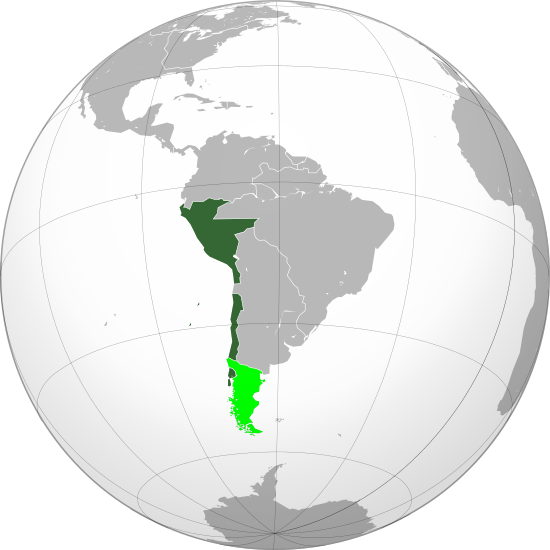
\includegraphics[width=\textwidth]{vice_peru.png}
\caption{\label{fig:1a}}
\end{subfigure}
\begin{subfigure}{0.15\textwidth}
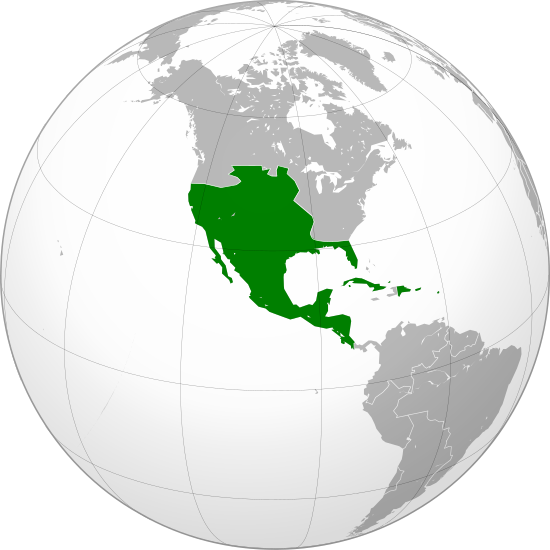
\includegraphics[width=\textwidth]{vice_nuevaespana.png}
\caption{\label{fig:1b}}
\end{subfigure}
\begin{subfigure}{0.15\textwidth}
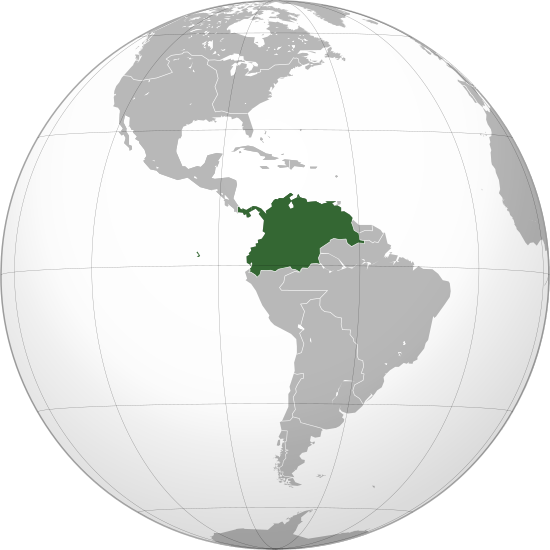
\includegraphics[width=\textwidth]{vice_nuevagranada.png}
\caption{\label{fig:1c}}
\end{subfigure}
\begin{subfigure}{0.15\textwidth}
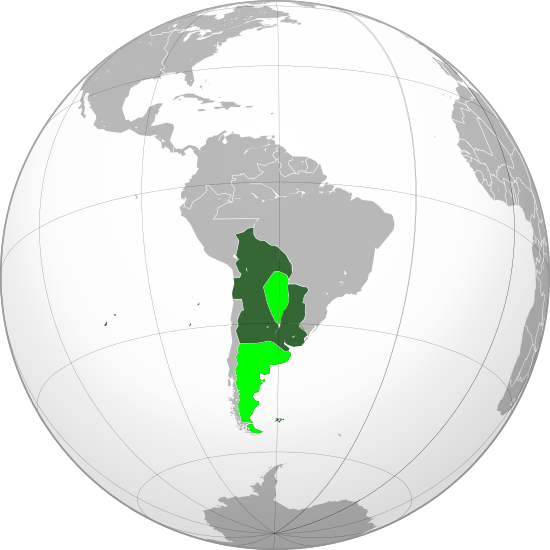
\includegraphics[width=\textwidth]{vice_riodelaplata.png}
\caption{\label{fig:1d}}
\end{subfigure}
\caption{\label{fig:1} Maps depicting \textit{virreinatos} in Latin America, 17th and 18th centuries.}
\end{figure}
\begin{table}[ht]
\small
\centering
\begin{tabular}{| c | c | c |}
\hline
\textbf{Map in Fig. \ref{fig:1}} (a-d) & \textbf{\textit{Virreinato}} & Captial $~~~~~~~~~~$ \\ \hline
& \textit{Nueva Espa\~{n}a} & $~~~~~~~~~~$ \\ \hline
& \textit{Nueva Granada} & $~~~~~~~~~~$ \\ \hline
& \textit{R\'{i}o de la Plata} & $~~~~~~~~~~$ \\ \hline
& \textit{Per\'{u}} & $~~~~~~~~~~$ \\ \hline
\end{tabular}
\caption{\label{tab:1} Fill in the missing information.}
\end{table}
\item Consider the library of Jos\'{e} Ignacio Bartolache.  (a) What does the distribution of texts in this library tell us about the scientific attitude of Latin Americans in the 18th Century? (b) What other scientific items did Bartolache own, and what clues does this add to our picture of the scientific attitude in that time and place?  (c) Considering these collections were built before 1760, draw a comparison to the state of science in the American colonies (later the United States). \\ \vspace{1cm}
\end{enumerate}

\section{Unit 1}

\begin{enumerate}
\item In Chapter 2 of \textit{The Scientific Attitude}, we encounter the following quote:
\begin{quotation}
Samir Okasha recounts the example of John Couch Adams and Urbain Le Verrier ... they were working (independently) within the Newtonian paradigm and noticed a slight perturbation in the orbit of the planet Uranus.
\end{quotation}
Newton's Law of Gravity predicts perfectly elliptical orbits for the planets, with no perturbations.  Was the law of gravity therefore \textit{falsified}?  What solved the problem in the end? \\ \vspace{0.5cm}
\item \textbf{Bode's Law} was an attempted mathematical explanation of the planetary orbits.  Bode's sequence was the pattern $0, 3, 6, 12, 24,...$, plus 4 to each, then divide the sequence by 10.  The result is 0.4, 0.7, 1.0, 1.6, 2.8, 5.2, 10.0, 19.6, 38.8, 77.2,... .  At the time (1772), the radii of the planets from the Sun were $0.387, 0.723, 1.0, 1.524, 5.203, 9.539$.  Nine years later, Uranus was discovered at 19.18.  Twenty years later, the asteroid belt between Mars and Jupiter was discovered at 2.77.  Did Bode's Law become a scientific fact because it fit the data? \\ \vspace{1cm}
\item In 1761, Judge Francisco Javier Gamboa created a set of legal and scientific studies that were meant to reform the mining industry, to make it more efficient.  Recall some scientific results that he shared within his \textit{Comentarios a las ordenanzas de minas}.  What chemicometallurgical technique, important for ore extraction, did he share with The Crown?  What institutions did he suggest creating? \\ \vspace{1.0cm}
\item \textit{El Real Seminario de Miner\'{i}a} was created by Joaqu\'{i}n Vel\'{a}zquez de Le\'{o}n, Fausto de Elh\'{u}yar, and others.  However, several factors might have driven it to bankrupcy.  Describe the Mexican efforts to preserve it. \\ \vspace{1.0cm}
\item What are the two tenets of the scientific attitude, or ethos, according to the author of \textit{The Scientific Attitude}? \\ \vspace{0.5cm}
\item Recall the story of Ignaz Semmelweis and antiseptic handwashing in maternity wards.  Discuss how the scientific attitude was applied in this situation. \\ \vspace{1cm}
\item Recall the story of the false discovery of cold fusion.  (a) Discuss how the scientific attitude was not applied in this situation. (b) Now select a piece of science from Latin American history that we have encountered thus far, and apply the criteria of the scientific attitude to it.  \\ \vspace{1cm}
\end{enumerate}

\section{Unit 2}
\begin{enumerate}
\item (a) In what viceroyalty (Fig. \ref{fig:1}) was the city of Santa Fe de Bogot\'{a}? (b) Discuss the scientific implications of the ``half century-long polemic on Copernican theories, which started in 1773 between Jos\'{e} Celestino Mutis and the Dominican Congregation of Santa Fe de Bogot\'{a}. (c) In 1783, the Expedici\'{o}n Bot\'{a}nica began in Santa Fe.  What were some of its goals and achievements? \\ \vspace{2cm}
\item (a) In what viceroyalty (Fig. \ref{fig:1}) was the city of Caracas? (b) In 1767, the Jesuit order was expelled from the Spanish colonies.  The Dominican order recovered authority over some colleges and universities.  What was the implication for science? \\ \vspace{2cm}
\item What scientific publication was created by Jos\'{e} Celestino Mutis? \\ \vspace{0.5cm}
\item Evaluate the logical truth of this claim: ``anti-vaccination campaigns do not have the scientific attitude, therefore these are not scientific endeavors.'' \\ \vspace{1cm}
\item Discuss one example we have encountered from our scientific history that should count as science, even though it has not traditionally been considered scientific. \\ \vspace{1cm}
\item In Chapter 3 of \textit{Science in Latin America}, we encounter the following quote:
\begin{quotation}
\textit{La Universidad Gegoriana} in Quito alone had ``seventy-one foreign professors teaching at the university ... Native professors were twenty-one, of whom five were from Loja, four from Quito, three from Guayas, three from Cuenca, three from Riobamba, two from Ibarra, and one from Ambato.'' ... As a consequence, it is not strange that in a center of cultural ferment such as Quito, intellectual Jesuits were most closely linked to the Franco-Spanish geodetic mission directed by La Condamine and Jorge Juan.
\end{quotation}
(a) What scientific transition began to take place as a result of the interaction between foreign and Ecuadorian professors? (b) What can we infer about the ratio of the native professors at the university? (c) Consider Father Fransisco Javier Aguilar, who taught physics and mathematics at Universidad Gregoriana.  He taught no less than five world systems, and focused on three: Ptolemaic, Copernican, and Tychonic.  What distinguished these? \\ \vspace{1cm}
\item In 1767, Mutis published \textit{Reflexiones sobre el sistema tyc\'{o}nico}. (a) What were the main points of this publication?  (b) Was it considered controversial? \\ \vspace{1cm}
\item When Joaqu\'{i}n Vel\'{a}zquez de Le\'{o}n and Jos\'{e} de G\'{a}lvez arrived in Baja California, they remained there for three years.  (a) What types of measurements did they make? (b) How did this improve local knowledge of Nueva Espa\~{n}a? (c) Vel\'{a}zquez de Le\'{o}n communicated with Chappe d'Auteroche that he would help with the Venus transit measurements, and d'Auteroche suggested that Vel\'{a}zquez de Le\'{o}n remain in Real de Santa Ana, while d'Auteroche would work in San Jos\'{e} del Cabo.  What happened as a result? \\ \vspace{1cm}
\item What was notable about the explorations of Jos\'{e} Sanchez Labrador? \\ \vspace{1cm}
\end{enumerate}

\section{Applications, Mayan and Incan Number Systems}

\begin{enumerate}
\item Work out the following exercises \textit{using the Mayan system.}
\begin{enumerate}
\item $365 + 365 = $ \vspace{1cm}
\item $1024 - 512 = $ \vspace{1cm}
\end{enumerate}
\item Work out the following exercises \textit{using the Incan quipu:}
\begin{enumerate}
\item $512 + 256 = $ \vspace{1cm}
\item $365 - 67 = $ \vspace{1cm}
\end{enumerate}
\item Suppose we are looking for a set of trees tall enough to supply sixteen four-meter beams.  Using the Mayan system, create a calculation showing that the total number of beams is sixty-four. \\ \vspace{2cm}
\item Suppose you have six terrace plots in the Andean mountains to use to survive.  You and your cohort of fellow Incans decide to grow potatoes and quinoa. Quinoa actually do better at higher altitudes that potatoes.  So the plan is to use the two lowest terraces for potatoes, and the upper four for quinoa.  Each terrace is 30 meters by 5 meters.  A potato plant requires a 0.2 meter by 0.2 meter patch, and a quinoa plant requires a 0.3 meter by 0.3 meter patch.  How many potato plants and how many quinoa plants can you plant? Store the results in a diagram of quipu knot system. \\ \vspace{2.5cm}
\end{enumerate}

\section{Modern Science in Latin America - Gamma Ray Astrophysics}

\begin{enumerate}
\item What is a gamma-ray?
\begin{itemize}
\item A: A charged particle with mass
\item B: A neutral particle with mass
\item C: A quantum of light
\item D: A radio wave
\end{itemize}
\item What was the purpose of the Milagro experiment?
\begin{itemize}
\item A: To observe the direction of incoming gamma-rays
\item B: To observe the energy of incoming gamma-rays
\item C: To observe the direction and energy of incoming gamma-rays
\item D: To observe the charge of incoming gamma-rays
\end{itemize}
\item What upgrades to the Milagro concept were made that produced the HAWC design?
\begin{itemize}
\item A: Using oil instead of water as the detection medium
\item B: Increasing the amount of water tanks to improve the sensitivity
\item C: Moving the tanks to a higher altitude
\item D: Both B and C
\end{itemize}
\item List some of the discoveries of HAWC and/or Milagro in the field of gamma-ray astrophysics. \\ \vspace{1cm}
\end{enumerate}

\section{Modern Science in Latin America - Cosmic Ray Physics}

\begin{enumerate}
\item What is the purpose of the Pierre Auger Observatory? \\ \vspace{1cm}
\item What is the typical energy of a cosmic-ray observed at Auger?
\begin{itemize}
\item A: $10^{12}$ eV
\item B: $10^{14}$ eV
\item C: $10^{16}$ eV
\item D: $10^{18}$ eV
\end{itemize}
\end{enumerate}

\end{document}
